\documentclass{beamer}
\usepackage{beamerthemeboxes}
\usepackage[utf8]{inputenc}
\usepackage{times}
\usepackage{palatino, url, multicol}

\mode<presentation>
{
  \usetheme{Warsaw}
  % or ...

  % or whatever (possibly just delete it)
   \usefonttheme[onlylarge]{structuresmallcapsserif}

    \usecolortheme{seahorse}

    \setbeamerfont{title}{shape=\itshape,family=\rmfamily}

}


\providecommand{\e}[1]{\ensuremath{\times 10^{#1}}}

\title[Strumenti Didattici per Embedded]{Sviluppo di Strumenti Didattici
per la Programmazione Embedded}
\author{Michele Bianchi}
\usepackage{graphicx}
\date{22 Settembre 2010}
\begin{document}
   \section{Introduzione}
	\frame{
		\titlepage
	}
   \subsection{Struttura}
	\frame{
		\frametitle{Introduzione}
 		\begin{block}{Difficoltà nella programmazione Embedded}
            \begin{itemize}
                \item Linguaggi di basso livello
                \item Difficoltà nel debugging
            \end{itemize}
        \end{block}
	    \begin{block}{Soluzione proposta}
            Collegamento tra il pacchetto di modellazione di sistemi
            discreti SciCos e il sistema embedded NXT 
        \end{block}
    }
   
   \subsection{NXT/SPAM}
   \frame{
        \frametitle{LEGO MINDSTORM NXT e SPAM}

            \begin{columns}
                \column{.40\textwidth}
                    \textbf{LEGO MINDSTORM NXT}

                    ~~~Piattaforma Embedded per la creazione di robot e
                    sistemi automatici.

                    \hspace{1\textheight}
                    \textbf{Caratteristiche}

                    \begin{itemize}
                    \item Piattaforma ATMEL AT91SAM7
                    \item Controller Bluetooth
                    \item Connessione USB
                    \item Bus I$^2$C
                    \end{itemize}

                \column{.05\textwidth}
                \column{.55\textwidth}
                    \begin{figure}[h]
                    \centering
                    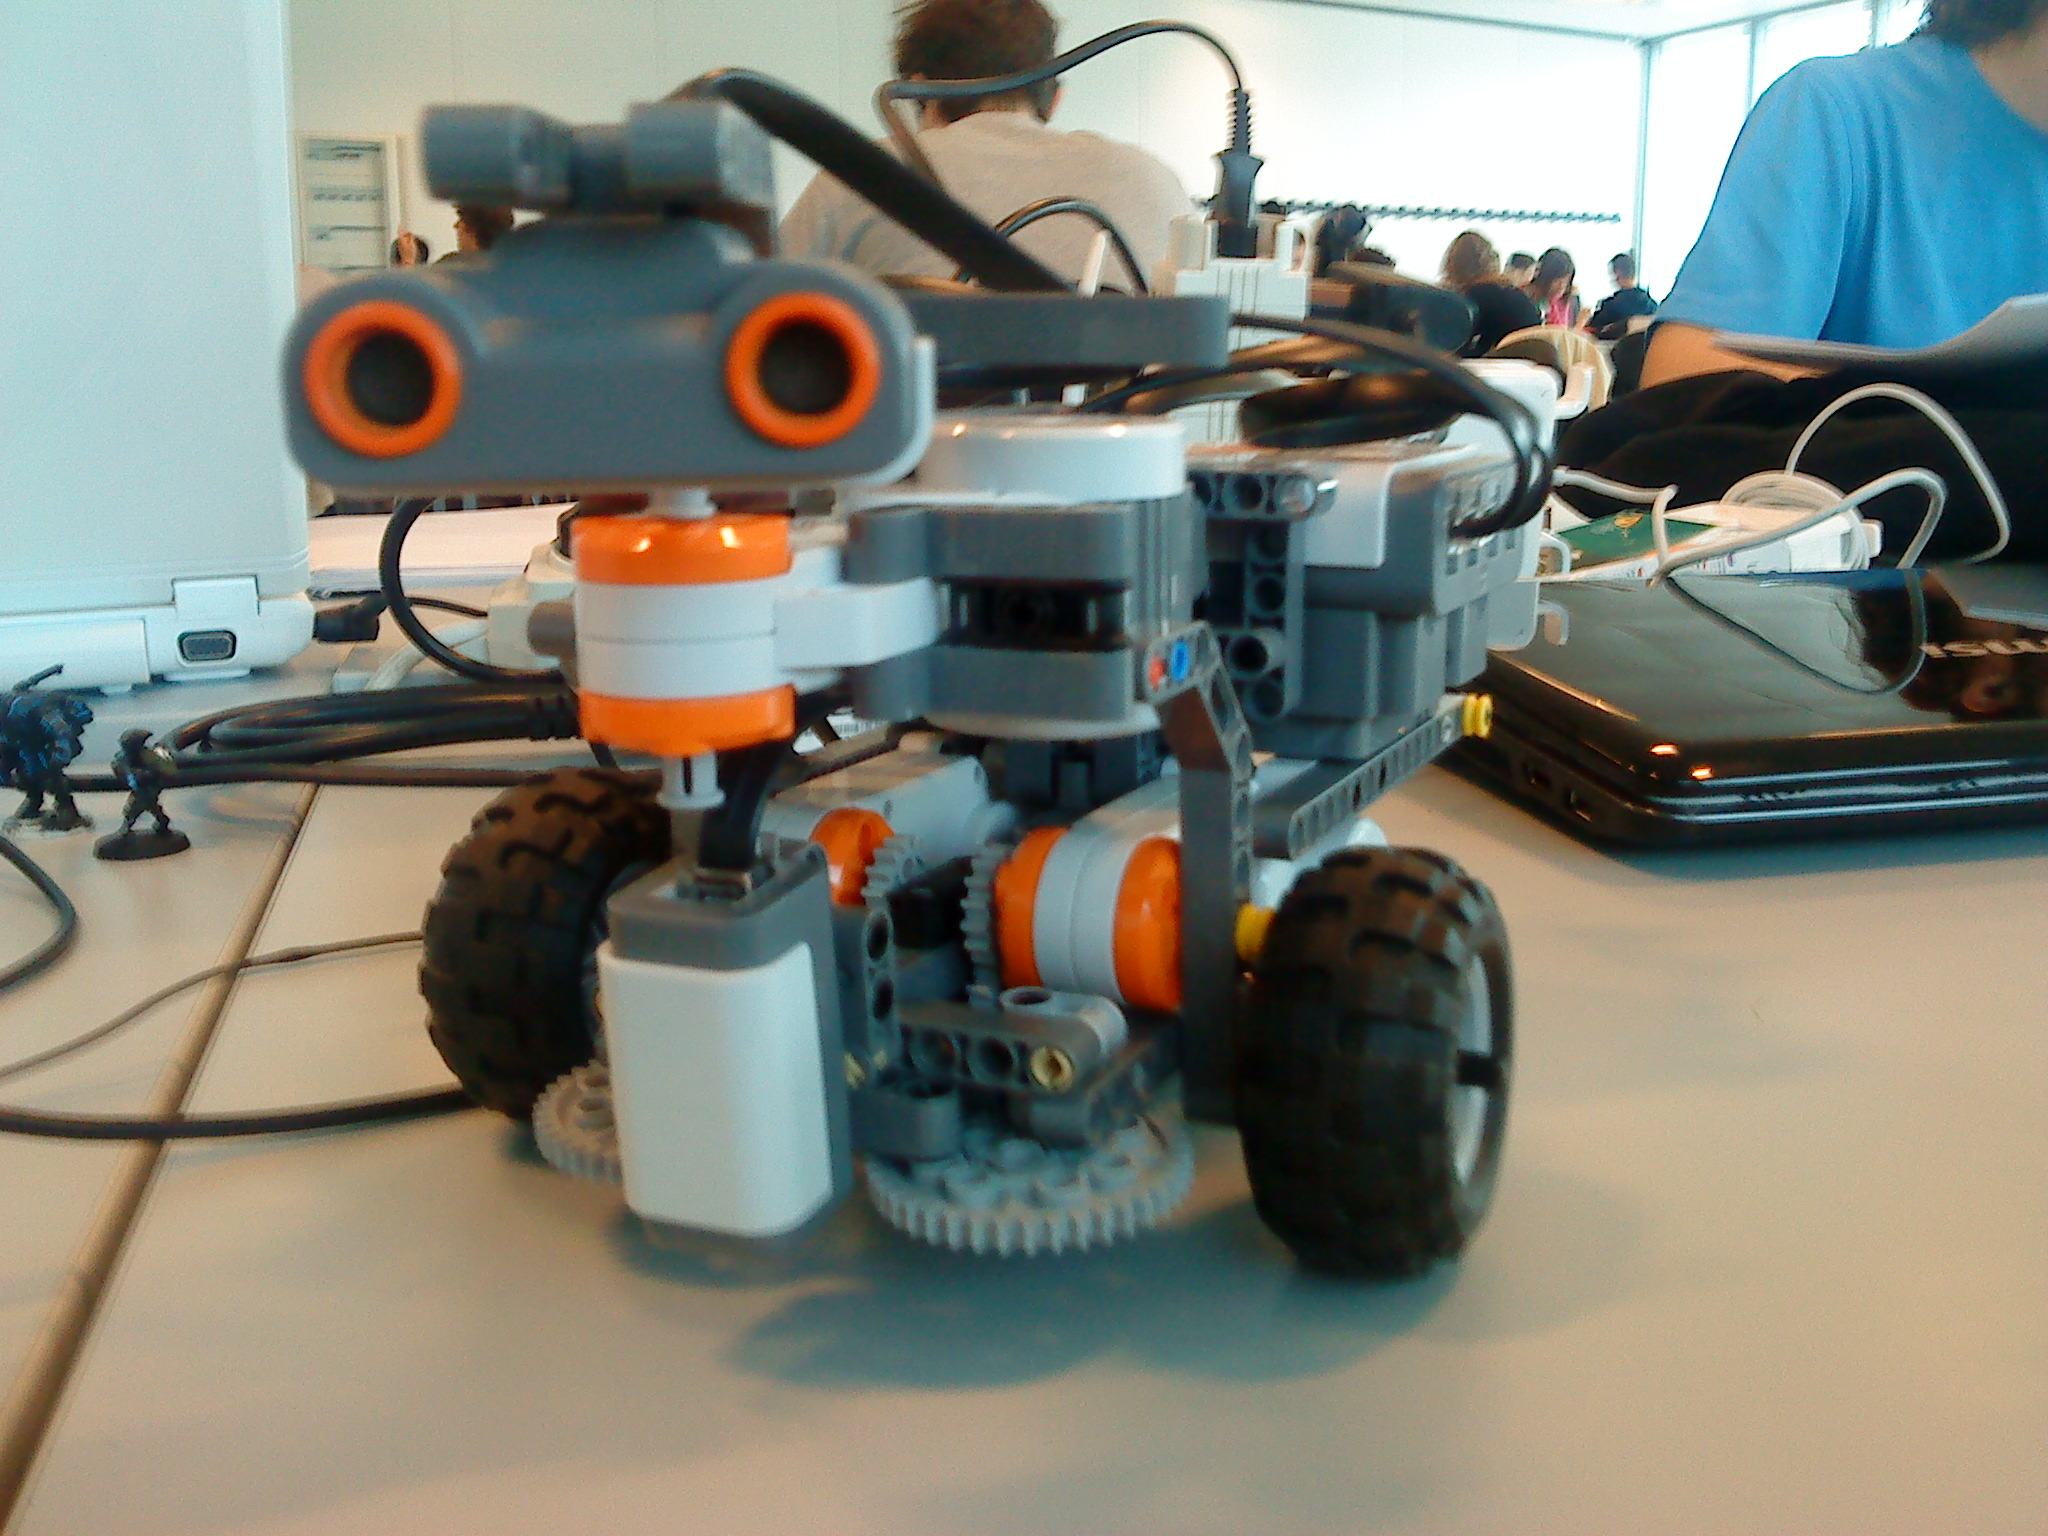
\includegraphics[scale=0.05]{../Pictures/SPAM.jpg}
                    \end{figure}

                    \begin{block}{SPAM}
                        \begin{itemize}
                         \item Due motori indipendenti
                         \item Sensore di luce
                         \item Sensore brandeggiabile di distanza 
                        \end{itemize}
                    \end{block}
            \end{columns}

   }


   \subsection{nxtOSEK}
	\frame{
		\frametitle{nxtOSEK}
        Sistema operativo per LEGO NXT
        \begin{block}{Features}
            \begin{itemize}
                \item Scritto in C
                \item Primitive OSEK/ATK e $\mu$Itron
                \item Device Drivers LeJOS NXJ
            \end{itemize}
        \end{block}
        \begin{block}{Alternative}
            \begin{itemize}
                \item nxOS
                \item NXC/NBC
            \end{itemize}
        \end{block}

    }

   \subsection{PID Controller}
    \frame{
        \frametitle{Digital PID Controller}
        \begin{block}{Caratteristiche}
           \begin{itemize}
            \item Sistema di controllo ciclico
            \item Cerca di minimizzare l'errore da iterazione ad iterazione
           \end{itemize}
        \end{block}

        \begin{block}{PID su SPAM}
            \begin{itemize}
             \item Utilizzato per il controllo dei Servo Motori
             \item Raggiunge la velocità richiesta dopo un breve periodo di
                oscillazione
             \item Più alta è la velocità obiettivo più lungo è il periodo
                di oscillazione
            \end{itemize}
        \end{block}
    }
   \section{Progetto}
    
    \frame{
        \title{Overview del progetto}

        \begin{itemize}
            \item Client eseguito su SPAM
            \item Applicazione Server che comunica col Client e con SciCos
            \item Blocchi d'interfaccia per SciCos
        \end{itemize}
    }

   \subsection{Client}
	\frame{
		\frametitle{Client}		
		\begin{itemize}
		    \item Riceve i comandi dal server
            \item Risponde a richieste sui sensori
            \item Contiene un PID Controller
            \item Stampa qualche dato a video
       \end{itemize}
       
       \begin{block}{Comunicazione col PC}
        \begin{itemize}
            \item Comunicazione USB tra nxtOSEK e PC problematica
            \item Scelta ricaduta sul Bluetooth
            \item Latenza alta $\sim{}45ms$
        \end{itemize}
       \end{block}
       
}
  \subsection{Population}
	\frame{
		\frametitle{Population Algorithm}
   	\begin{block}{Funzionamento:}
		\begin{itemize}
		\item ogni nodo parte con un token
		\item ad ogni incontro viene scelto un nodo (probabilità 50/50)
		\item il nodo scelto prende possesso dei token dell'altro
	    	\item alla fine i token finiscono in un unico nodo
		\item i nodi tengono memoria del numero massimo di token incontrati
	  	\end{itemize}
	\end{block}
	}
	\frame{
		\frametitle{C-Population Algorithm}
   \begin{block}{Caratteristiche:}
	\begin{itemize}
	 \item variazione di Population Algorithm
	 \item probabilità di assegnamento proporzionale all'attività
  	\end{itemize}
   \end{block}
	\begin{block}{Conseguenze}
	\begin{itemize}
	 \item i token finiscono nei nodi più attivi
    \item maggiore velocità di convergenza
	\end{itemize}
	\end{block}
	}
   \subsection{Two Phases}
	\frame{
		\frametitle{Two Phases Algorithm}
		\begin{block}{Caratteristiche:}
	\begin{itemize}
	 \item variazione di C-Population Algorithm
	 \item interviene in caso di stallo di C-Population
	 \item estrae e firma i token
	 \item diffonde le coppie (id-token)
  	\end{itemize}
\end{block}
	 \begin{block}{Conseguenze:}
	\begin{itemize}
	 \item aumento di traffico
	 \item maggiore robustezza
	 \item migliori performance
  	\end{itemize}
\end{block}
	}
   \section{Prestazioni}
   \subsection{Random Way Mobility}
	\frame{
		\frametitle{Risultati sul modello Random Way Mobility}
		\begin{block}{Caratteristiche del modello:}
		\begin{itemize}
		\item nodi in movimento in un playground
		\item attività uniforme
		\end{itemize}
		\end{block}
		\begin{block}{Tempi di convergenza medi}
\begin{center}		\begin{tabular}{|c||c|}
			\hline
			\textbf{Pairwise Averaging} &\textbf{Population}\\ 
			\hline
			 $ 8.00\pm0.00\e3 s$   & $ 2.10\pm0.23\e5 s$\\  
			\hline
			\hline
			\textbf{C-Population} & \textbf{Two-Phases}\\
			\hline
			$ 2.06\pm0.24\e5 s$  & $2.21\pm0.09\e4 s$\\ 
			\hline
		\end{tabular}
\end{center}		\end{block}
		\begin{block}{Considerazioni}
	\begin{itemize}
		\item Pairwise Averaging è il più veloce
		\item C-Population non guadagna rispetto a Population
	\end{itemize}
		\end{block}
	}
   \subsection{Reality Mining}
	\frame{
		\frametitle{Risultati sulla traccia Reality Mining}
		\begin{block}{Caratteristiche della traccia:}
		\begin{itemize}
		\item registrata dal MIT  
		\item attività poco uniforme
		\end{itemize}
		\end{block}
		\begin{block}{Tempi di convergenza medi}
\begin{center}		\begin{tabular}{|c||c|}
			\hline
			\textbf{Pairwise Averaging} &\textbf{Population}\\ 
			\hline
			  $ 2.47\pm0.16\e8 ms$   & $ 2.19\pm0.40\e9 ms$\\  
			\hline
			\hline
			\textbf{C-Population} & \textbf{Two-Phases}\\
			\hline
			$ 2.16\pm0.19\e7 ms$  & $2.24\pm0.05\e7 ms$\\ 
			\hline
		\end{tabular}
\end{center}		\end{block}
		\begin{block}{Considerazioni}
	\begin{itemize}
		\item C-Population diventa il più veloce
		\item Pairwise Averaging soffre la differenza di attività
	\end{itemize}
		\end{block}
	}
   \subsection{Perdita di messaggi}
	\frame{
		\frametitle{Effetti della perdita di messaggi}
		\begin{block}{Sviluppo di un incontro}
			\begin{enumerate}
				\item Nodo 1 manda i suoi dati
				\item Nodo 2 riceve e risponde
				\item Nodo 2 esegue l'algoritmo
				\item Nodo 1 riceve ed esegue l'algoritmo
			\end{enumerate}
		\end{block}
		\begin{itemize}
			\item Se si perde il messaggio di risposta l'algoritmo viene eseguito solo su un nodo.
			\item Si creano degli errori nella stima
		\end{itemize}
	}
	\frame{
		\frametitle{Pairwise Averaging su Random Way Mobility}
		\begin{figure}
		\begin{center}
		\includegraphics[scale=0.45]{aggr.png}
		\end{center}
		\end{figure}
	}
   \subsection{Conclusioni}
	\frame{
		\frametitle{Conclusioni ottenute}
		\begin{block}{Conclusioni:}
		\begin{itemize}
			\item Two-Phases e Pairwise Averaging sono i più robusti
			\item Pairwise Averaging più veloce in reti uniformi
			\item Two-Phases più veloce in reti non uniformi
			\item C-Population poco robusto, ma veloce in reti non uniformi
		\end{itemize}
		\end{block}
	}
\end{document}
